%%%%%%%%%%%%%%%%%%%%%%%%%%%%%%%%%%%%%%%
% Deedy CV/Resume
% XeLaTeX Template
% Version 1.0 (5/5/2014)
%
% This template has been downloaded from:
% http://www.LaTeXTemplates.com
%
% Original author:
% Debarghya Das (http://www.debarghyadas.com)
% With extensive modifications by:
% Vel (vel@latextemplates.com)
%
% License:
% CC BY-NC-SA 3.0 (http://creativecommons.org/licenses/by-nc-sa/3.0/)
%
% Important notes:
% This template needs to be compiled with XeLaTeX.
%
%%%%%%%%%%%%%%%%%%%%%%%%%%%%%%%%%%%%%%

\documentclass[a4paper]{deedy-resume} % Use US Letter paper, change to a4paper for A4 

\usepackage{wrapfig}
\usepackage{graphicx}
\usepackage{fontawesome5}

\graphicspath{ {images/} }

% ----  Skill bars ----
\usepackage{xcolor}
\definecolor{noskillgray}{gray}{0.85}
\definecolor{skilledblue}{rgb}{0.5,0.7,1}


\makeatletter
\newdimen\skillb@level
\newdimen\skillb@length
\newdimen\skillb@height
\skillb@length=120pt%
\skillb@height=10pt%
\newcommand*{\skillbar}[1]{%
    \skillb@level=\dimexpr#1\skillb@length/100\relax%
    {\color{skilledblue}\rule{\skillb@level}{\skillb@height}}%
    {\color{noskillgray}%
        \rule{\dimexpr\skillb@length-\skillb@level\relax}{\skillb@height}}%
}
\newcommand*{\skill}[2]{%
    \par\noindent%
    {\hskip 1ex\small #1}\\%
    \skillbar{#2}%
}
\makeatother


\begin{document}

%\begin{minipage}{0.33\textwidth}
%\end{minipage}
%\begin{minipage}{0.67\textwidth}

%----------------------------------------------------------------------------------------
%	TITLE SECTION
%----------------------------------------------------------------------------------------

%\lastupdated % Print the Last Updated text at the top right
%\begin{minipage}{0.1\textwidth}
%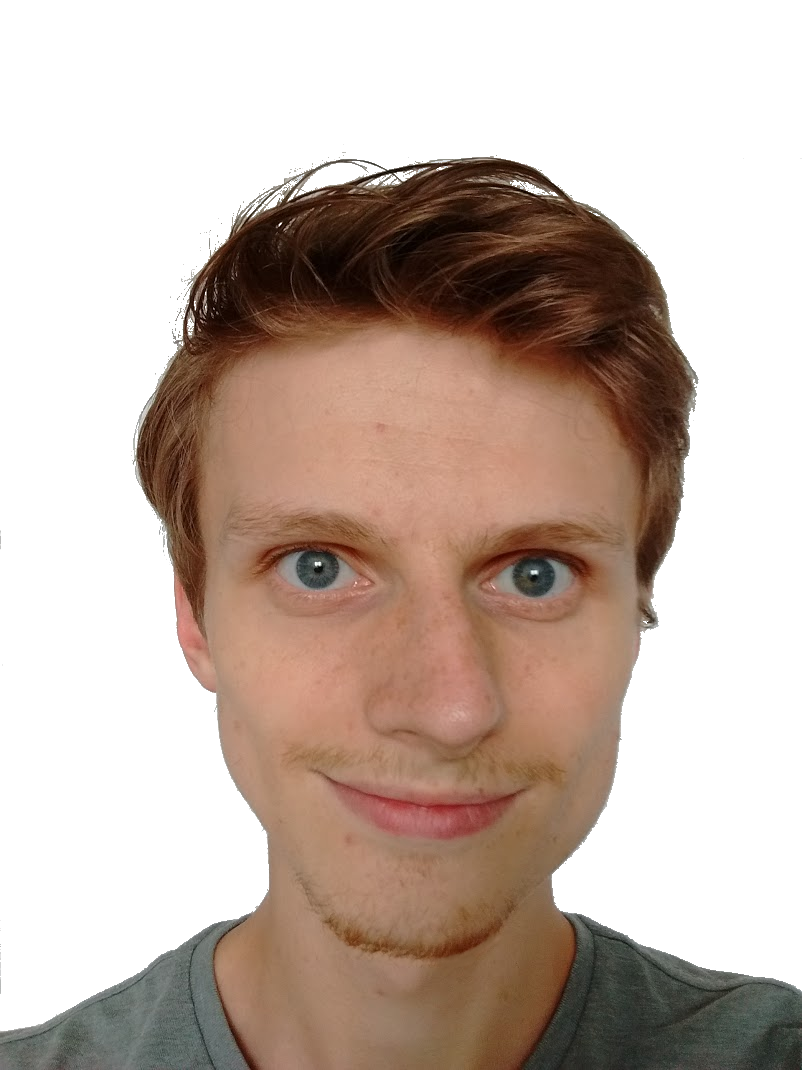
\includegraphics[width=\textwidth]{pic}
%\end{minipage}

\begin{minipage}{1\textwidth}


\namesection{}{Michaël de Vries}{ % Your name
% \urlstyle{same}\url{http://debarghyadas.com} \\ % Your website, LinkedIn profile or other web address

\faEnvelope  \hspace{0.2em}\href{mailto:vriesdemichael+cv@gmail.com}{vriesdemichael@gmail.com} | \faPhone \hspace{0.2em} (+31) 6 54938929 
	\\ \faHome \hspace{0.2em} Almelo, The Netherlands | \faLinkedin \hspace{0.2em} \href{www.linkedin.com/in/vriesdemichael}{vriesdemichael}

}
\end{minipage}
\\
%\rule{\paperwidth}{0.4pt}

\noindent\makebox[\linewidth]{\color{headings}\rule{\paperwidth}{0.4pt}} % Horizontal rule
\vspace{-5pt} % Reduce whitespace after the rule slightly



%----------------------------------------------------------------------------------------
%	LEFT COLUMN
%----------------------------------------------------------------------------------------

\begin{minipage}[t]{0.33\textwidth} % The left column takes up 33% of the text width of the page

%------------------------------------------------
% Education
%------------------------------------------------
%\section{}
\vspace{0em}
%\begin{center}
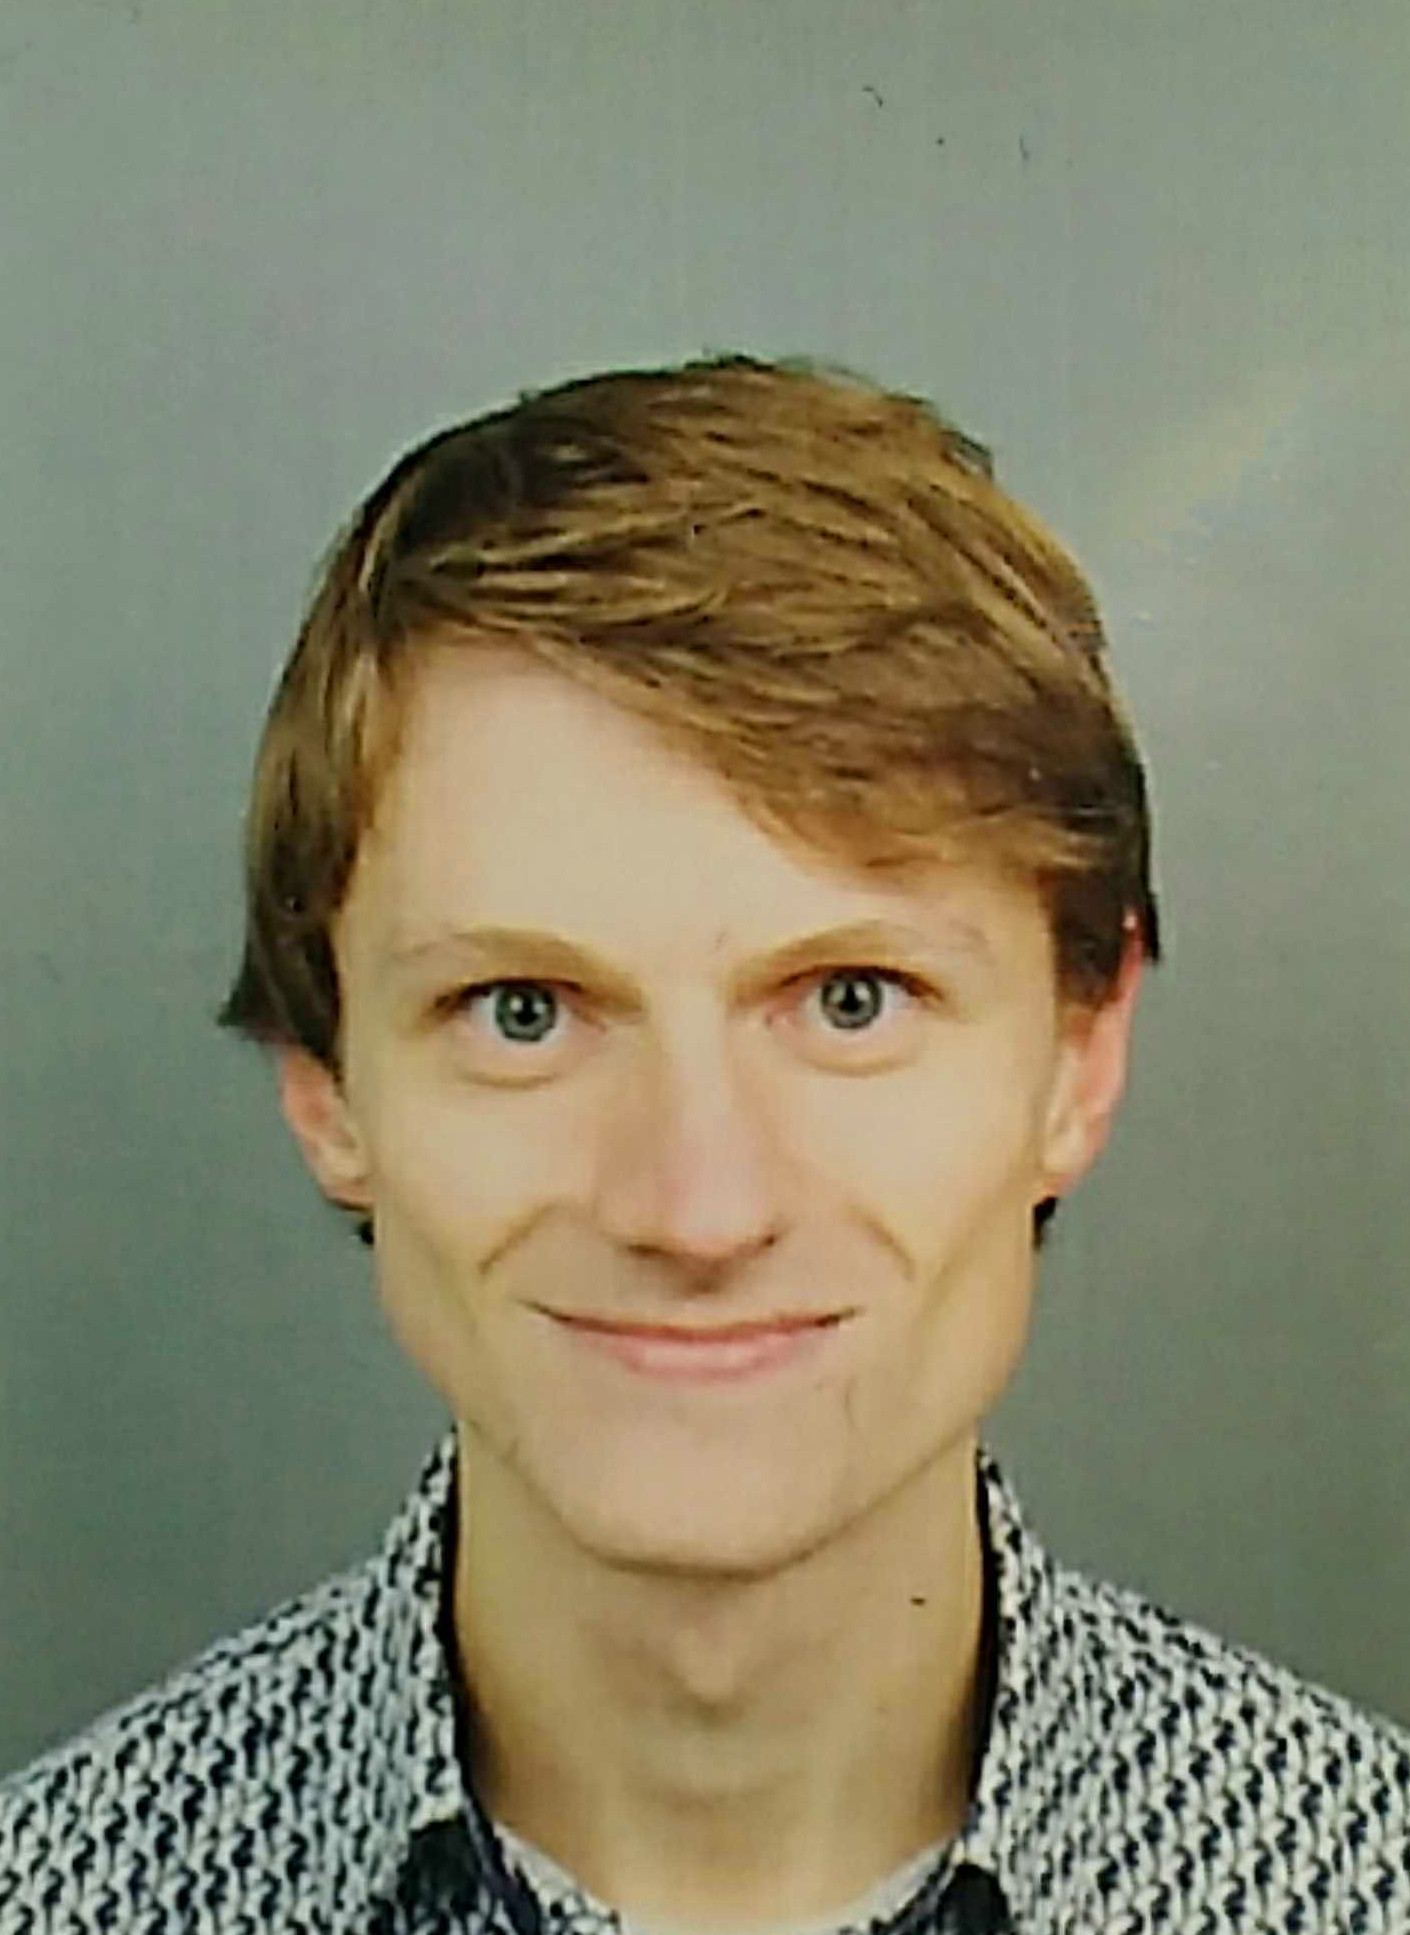
\includegraphics[width=0.9\textwidth]{pic3}
%\end{center}

\section{Education} 

\subsection{University of Twente}
\descript{Premaster computer science}
\location{Sep 2017 -  Apr 2018 | Enschede 
	\\ Premaster as minor of bachelor
}
\sectionspace % Some whitespace after the section

%------------------------------------------------


\subsection{Saxion university of applied sciences}
\descript{Bachelor computer science}
\location{Expected Nov 2018 | Enschede 
	\\ Incl. 30EC in big data electives
    }
\sectionspace % Some whitespace after the section

%------------------------------------------------
% Links
%------------------------------------------------

% \section{Links} 

% Github:// \href{https://github.com/deedydas}{\bf deedydas} \\
% LinkedIn:// \href{https://www.linkedin.com/in/debarghyadas}{\bf debarghyadas} \\
% YouTube:// \href{https://www.youtube.com/user/DeedyDash007}{\bf DeedyDash007} \\
% Twitter:// \href{https://twitter.com/debarghya_das}{\bf @debarghya\_das} \\
% Quora:// \href{https://www.quora.com/Debarghya-Das}{\bf Debarghya-Das}


%------------------------------------------------
% Skills
%------------------------------------------------

\section{Skills}

\subsection{\faFlask \hspace{0.2em} Data science}
\skill{Model development}{80}
\skill{ETL}{30}
\skill{Visualization}{60}
\skill{Deployment}{70}

\sectionspace % Some whitespace after the section


\subsection{\faCode \hspace{0.2em}  Programming}
\skill{Python}{95}
\skill{Java}{60}
%\skill{C}{50}
%\skill{Scala}{40}


\sectionspace
%----------------------------------------------------------------------------------------

\subsection{\faTools \hspace{0.2em} tools} 
\location{Linux (CentOS, Redhat, Ubuntu), TensorFlow, Keras, PyTorch, Jupyter, Docker, Bash, Apache Flink, Apache Spark, OSGi, Redis}



\end{minipage} % The end of the left column
\hfill
%
%----------------------------------------------------------------------------------------
%	RIGHT COLUMN
%----------------------------------------------------------------------------------------
%
\begin{minipage}[t]{0.62\textwidth} % The right column takes up 66% of the text width of the page

%------------------------------------------------
% Experience
%------------------------------------------------



\section{Experience}

\runsubsection{Belastingdienst}
\descript{| Data science developer/engineer}

\location{Jan 2019 – Now | Apeldoorn}
\vspace{\topsep} % Hacky fix for awkward extra vertical space

\begin{tightitemize}
\item Train and implement machine learning models for various NLP tasks.
\item Framework development for model deployment.
\item Role as scrum master.
\end{tightitemize}

\sectionspace % Some whitespace after the section



\runsubsection{Luminis}
\descript{| Data science intern }

\location{May 2018 – Nov 2018 | Apeldoorn}
%\vspace{\topsep} % Hacky fix for awkward extra vertical space

\begin{tightitemize}
\item Final internship in year 4 of the Bsc, graded 9.
\item Trained a deep learning model for product categorization based on images of products.
\item Created an interface for AI assisted product categorization using the trained model.
\item Model (and interface) deployment in a docker container.
\end{tightitemize}

\sectionspace % Some whitespace after the section


\runsubsection{Thales}
\descript{| Software developer intern}

\location{Sep 2016 – Feb 2017 | Hengelo}
%\vspace{\topsep} % Hacky fix for awkward extra vertical space

\begin{tightitemize}
\item First internship in year 2 of the Bsc, graded 9.
\item Developed a python interpreter which works within a multithreaded OSGi framework programmed in C.
\item Work involved writing interoperable software in C and Python.
\end{tightitemize}

\sectionspace % Some whitespace after the section

%------------------------------------------------

\runsubsection{Comyoo}
\descript{| Web developer}

\location{Sep 2014 – Oct 2015 | Enschede}
%\vspace{\topsep} % Hacky fix for awkward extra vertical space
\begin{tightitemize}
\item Part-time job during bachelor.
\item Web development using Angular in combination with Joomla.
\end{tightitemize}

\sectionspace % Some whitespace after the section


%------------------------------------------------
% Projects
%------------------------------------------------

\section{Projects}

\runsubsection{Premaster Research}
\descript{| Human media interaction}
\location{Sep 2017 - Feb 2018 | 10EC | University of Twente}
A research on \textbf{speech emotion recognition} for the human media interaction section of the university of Twente. The research used speech fragments annotated with the emotions exhibited in the fragments by multiple annotators. The acoustic features of the speech fragments were analyzed to find discriminative features for a low level of agreement between annotators.

\sectionspace

\runsubsection{Data streaming}
\descript{| JW Player}
\location{Feb 2016 - Jun 2016 | 12EC | Saxion university of applied sciences}
A group project in cooperation with two data scientist at JW Player. JW Player uses a \textbf{lambda architecture} for their video log processing, we were assigned to create a new branch in the \textbf{real-time processing} system. We implemented a \textbf{Apache Flink} streaming system which gave the top 10 topics of videos played in the past minute. To do so we implemented \textbf{topic modeling} using the stanford NPL package and trained a model based on data of the previous hour.

The system was connected to \textbf{kafka} and wrote to a \textbf{redis} database, all of which we hosted on a \textbf{AWS cluster}.

\sectionspace

%\runsubsection{WiFi tracking}
%\descript{| Saxion/Municipality of Enschede/NDIX}
%\location{Feb 2015 - Jun 2016 | 12EC | Saxion university of applied sciences}
%This was the first big project of the bachelor computer science. A tracking system for visitors of the inner city of Enschede was made based on the logs of an open WiFi network with multiple access points in the shopping district. We created an algorithm to determine coordinates of visitors based on signals received by the access points. As a visualization for the municipality we made an HTML front-end using \textbf{CartoDB} with heat maps, routes and statistics for every hour of any given day.


%------------------------------------------------
% Research
%------------------------------------------------

%\section{Research}
%
%\runsubsection{Cornell Robot Learning Lab}
%\descript{| Head Undergrad Research}
%
%\location{Jan 2014 – Present | Ithaca, NY}
%Worked with \textbf{\href{http://www.cs.cornell.edu/~ashesh/}{Ashesh Jain}} and \textbf{\href{http://www.cs.cornell.edu/~asaxena/}{Prof Ashutosh Saxena}} to create \textbf{PlanIt}, a tool which learns from large scale user preference feedback to plan robot trajectories in human environments. Publication submitted.
%
%\sectionspace % Some whitespace after the section
%
%%------------------------------------------------
%
%\runsubsection{Cornell Phonetics Lab}
%\descript{| Head Undergraduate Researcher}
%
%\location{Mar 2012 – May 2013 | Ithaca, NY}
%Lead the development of \textbf{QuickTongue}, the first ever breakthrough tongue-controlled game with \textbf{\href{http://conf.ling.cornell.edu/~tilsen/}{Prof Sam Tilsen}} to aid in Linguistics research. Publication submitted.
%
%\sectionspace % Some whitespace after the section
%
%%------------------------------------------------
%% Awards
%%------------------------------------------------
%
%\section{Awards} 
%
%\begin{tabular}{rll}
%2014	 & top 52/2500 & KPCB Engineering Fellow\\
%2014	 & 2\textsuperscript{nd} most points & Google Code Jam, Qualification Round\\
%2014	 & 1\textsuperscript{st}/50 & Microsoft Coding Competition, Cornell\\
%2013	 & National & Jump Trading Challenge Finalist\\
%2013 & 7\textsuperscript{th}/120 & CS 3410 Cache Race Bot Tournament \\
%2012 & 2\textsuperscript{nd}/150 & CS 3110 Biannual Intra-Class Bot Tournament \\
%2011 & National & Indian National Mathematics Olympiad (INMO) Finalist \\
%2010 & National & Comp. Soc. of India's National Programming Contest\\
%\end{tabular}
%
%\sectionspace % Some whitespace after the section

%------------------------------------------------
% Societies
%------------------------------------------------

%\section{Societies} 
%
%\begin{tabular}{rll}
%2014 & top 12\%ile & Tau Beta Pi Engineering Honor Society\\
%2014 & National & The Global Leadership and Education Forum (tGELF)\\
%2012 & National & Golden Key International Honor Society\\
%2012 & National & National Society of Collegiate Scholars\\
%\end{tabular}
%
%\sectionspace % Some whitespace after the section

%----------------------------------------------------------------------------------------

\end{minipage} % The end of the right column

%----------------------------------------------------------------------------------------
%	SECOND PAGE (EXAMPLE)
%----------------------------------------------------------------------------------------

%\newpage % Start a new page

%\begin{minipage}[t]{0.33\textwidth} % The left column takes up 33% of the text width of the page

%\section{Example Section}

%\end{minipage} % The end of the left column
%\hfill
%\begin{minipage}[t]{0.66\textwidth} % The right column takes up 66% of the text width of the page

%\section{Example Section 2}

%\end{minipage} % The end of the right column

%----------------------------------------------------------------------------------------

\end{document}